% !TeX spellcheck = cs_CZ

\begin{example}\label{mai:exam004}
  \textbf{Parametrická vyjádření roviny}:\newline
  Rovina v trojrozměrném prostoru \(\mathcal{R}^3\) je zadána třemi body \(A\), \(B\) a \(C\), 
  které nesmějí ležet v jedné přímce, popřípadě dvěma body \(A\) a \(B\) a vektorem v nerovnoběžným 
  s \(\overrightarrow{AB}\), anebo bodem \(A\) a dvěma nerovnoběžnými směrovými vektory \(\vec{u}\) 
  a \(\vec{u}\) (obr. \ref{MAI:FIG002}). Všechny tyto typy zadání jsou ekvivalentní. Lze volit 
  například \(\vec{u} = \overrightarrow{AB}\), \(\vec{v} = \overrightarrow{AC}\). Je-li \(X\) 
  libovolným bodem roviny \(\varrho\), jsou vektory \(\overrightarrow{AX}\), \(\vec{u}\) a 
  \(\vec{v}\) \textbf{lineárně závislé}. To znamená, že existují taková reálná čísla \(r\) a \(s\), 
  že vektor \(\overrightarrow{AX}\) lze zapsat jako lineární kombinaci

  {\centering
    \captionsetup{type=figure}
    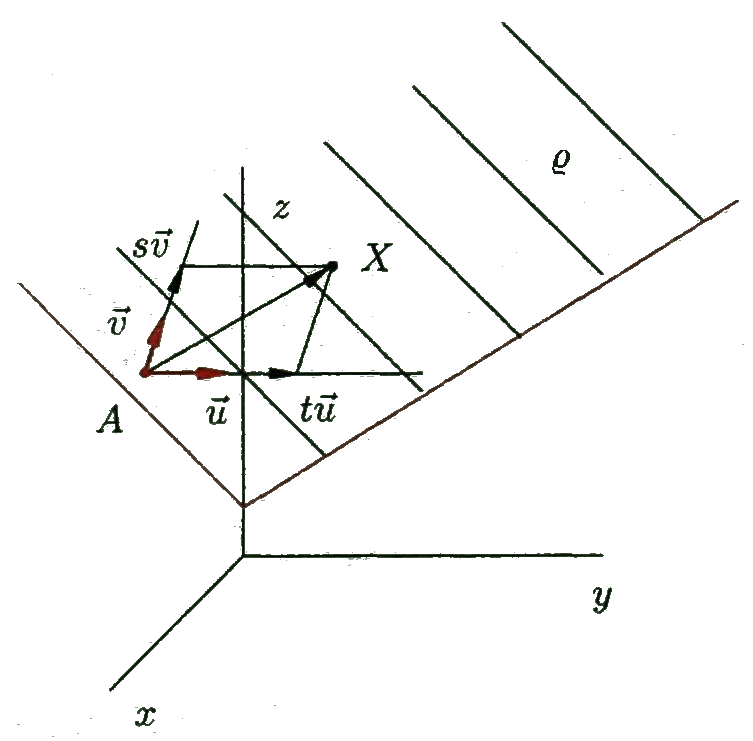
\includegraphics[width=0.5\linewidth]{Musilova_FIG002.png}
    \captionof{figure}{Zadáni roviny. \cite[s.~3]{Musilova2009MA1}}
    \label{MAI:FIG002}
    \par}  
  
\end{example}
  